\section{Оценка эффективности}
В рамках оценки эффективности разработанного программного комплекса проведём несколько серий экспериментов с его помощью, а затем осуществим анализ экспериментальных данных.

Далее в этом разделе мы последовательно рассмотрим следующие серии экспериментов и их анализ:
\begin{itemize}
    \item серия экспериментов по проверке точности измерения времени;
    \item серия экспериментов по сравнению производительности программ, собранных компиляторами \textit{GCC} и \textit{LLVM} на настройках <<по умолчанию>>;
    \item группа серий экспериментов по моделированию и предсказанию производительности программы из набора \textit{Polybench} на различном аппаратном обеспечении:
    \begin{itemize}
        \item серия экспериментов по моделированию и предсказанию производительности при размере входных данных, который меняется по степенному закону, а обе размерности входных данных одинаковы;
        \item серия экспериментов по моделированию и предсказанию производительности при размере входных данных, который меняется случайно при равномерном распределении случайной величины, а обе размерности входных данных одинаковы;
        \item серия экспериментов по моделированию и предсказанию производительности при размере входных данных, который меняется случайно при равномерном распределении случайной величины, а размерности входных данных не одинаковы.
    \end{itemize}
\end{itemize}

\subsection{Серия экспериментов по проверке точности измерения времени}
\label{ssec:series-accuracy}
Для проверки точности измерения времени проведём следующий эксперимент.

Сгенерируем семейство программ, которые не делают ничего, кроме вызова функции стандартной библиотеки \textit{C} \texttt{usleep}. Аргументами функции будет число $10^n$, где $n$ "--- число от одного до шести включительно. Таким образом, после запуска программа устанавливает таймер на заданное число микросекунд (от 1 мкс до 1000000 мкс = 1~с), останавливается и после его срабатывания завершает работу.

Далее на рис. \ref{img:calibration} приведён график измеренного времени исполнения семейства таких программ и <<реального>> времени их выполнения "--- т.е. времени, указанного в аргументе функции, создающей таймер. График построен с помощью инструментария в автоматическом режиме.

\begin{figure}[p]
    \center{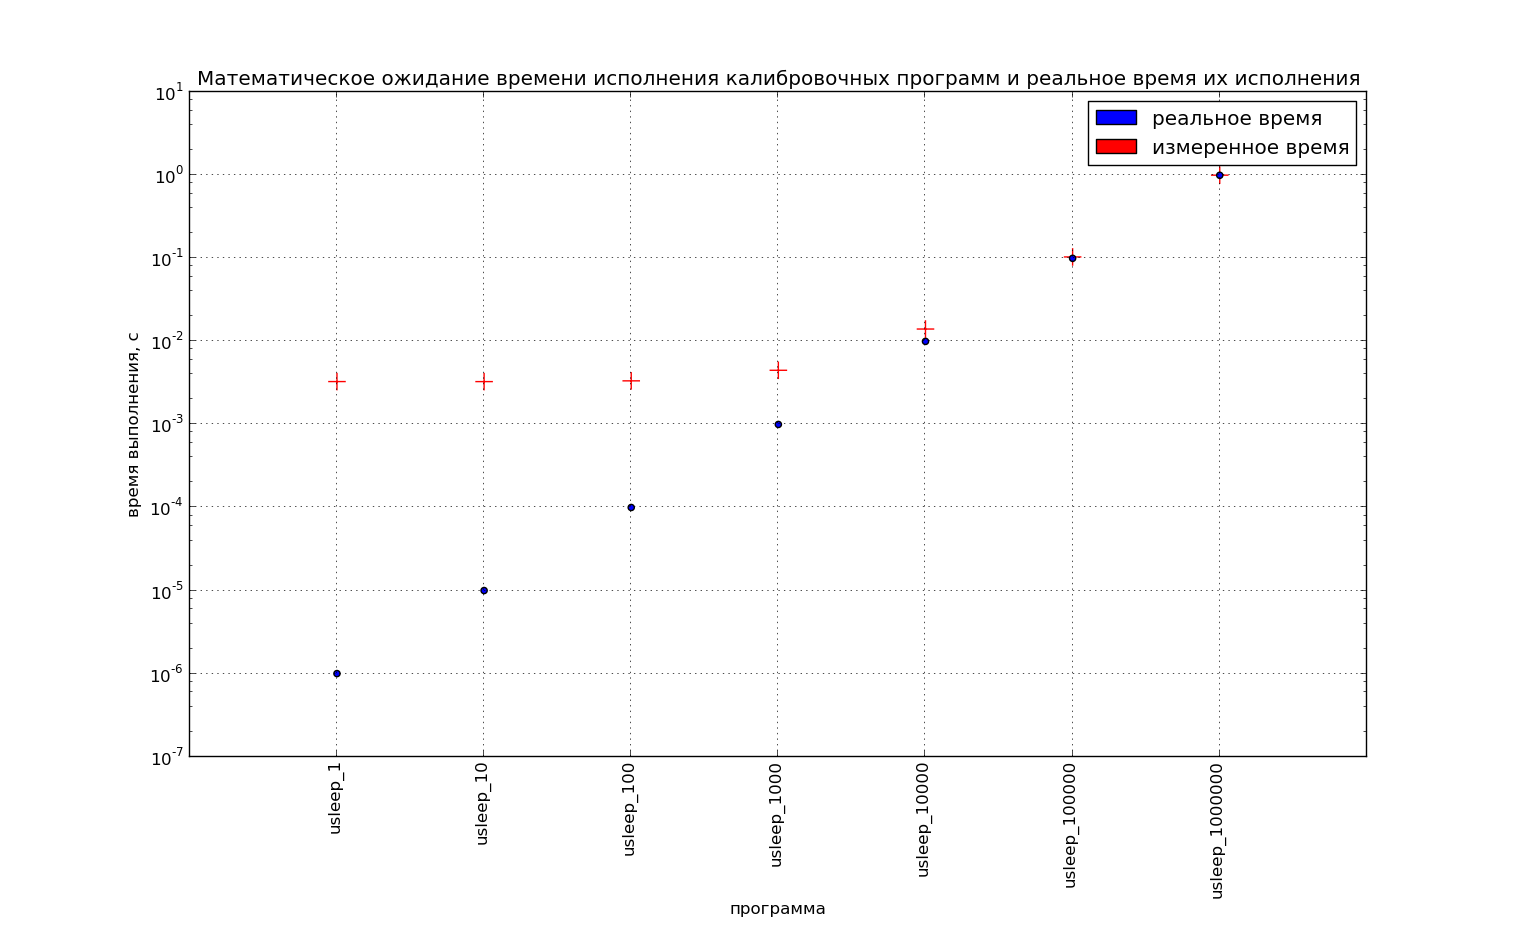
\includegraphics[width=1\linewidth]{calibration}}
    \caption{График измеренного и реального времени исполнения семейства калибровочных программ}
    \label{img:calibration}
\end{figure}

Как мы видим на рис. \ref{img:calibration}, измеренное время асимптотически приближается к значению между $10^{-2}$ и $10^{-3}$ "--- около 0,005.

Из этого можно сделать вывод, что существуют постоянные расходы на запуск программы из нашей системы и их можно вычесть из измеренного времени для повышения точности измерения. Для этого мы вычисляем время выполнения пустой программы (согласно описанной в подразделе~\ref{sssect:calibration} методике), а затем вычитаем его из каждого измеренного результата выполнения реальных программ.

На рис. \ref{img:calibration-offset} показан график измеренного времени в данном эксперименте с учётом накладных расходов.

\begin{figure}[p]
    \center{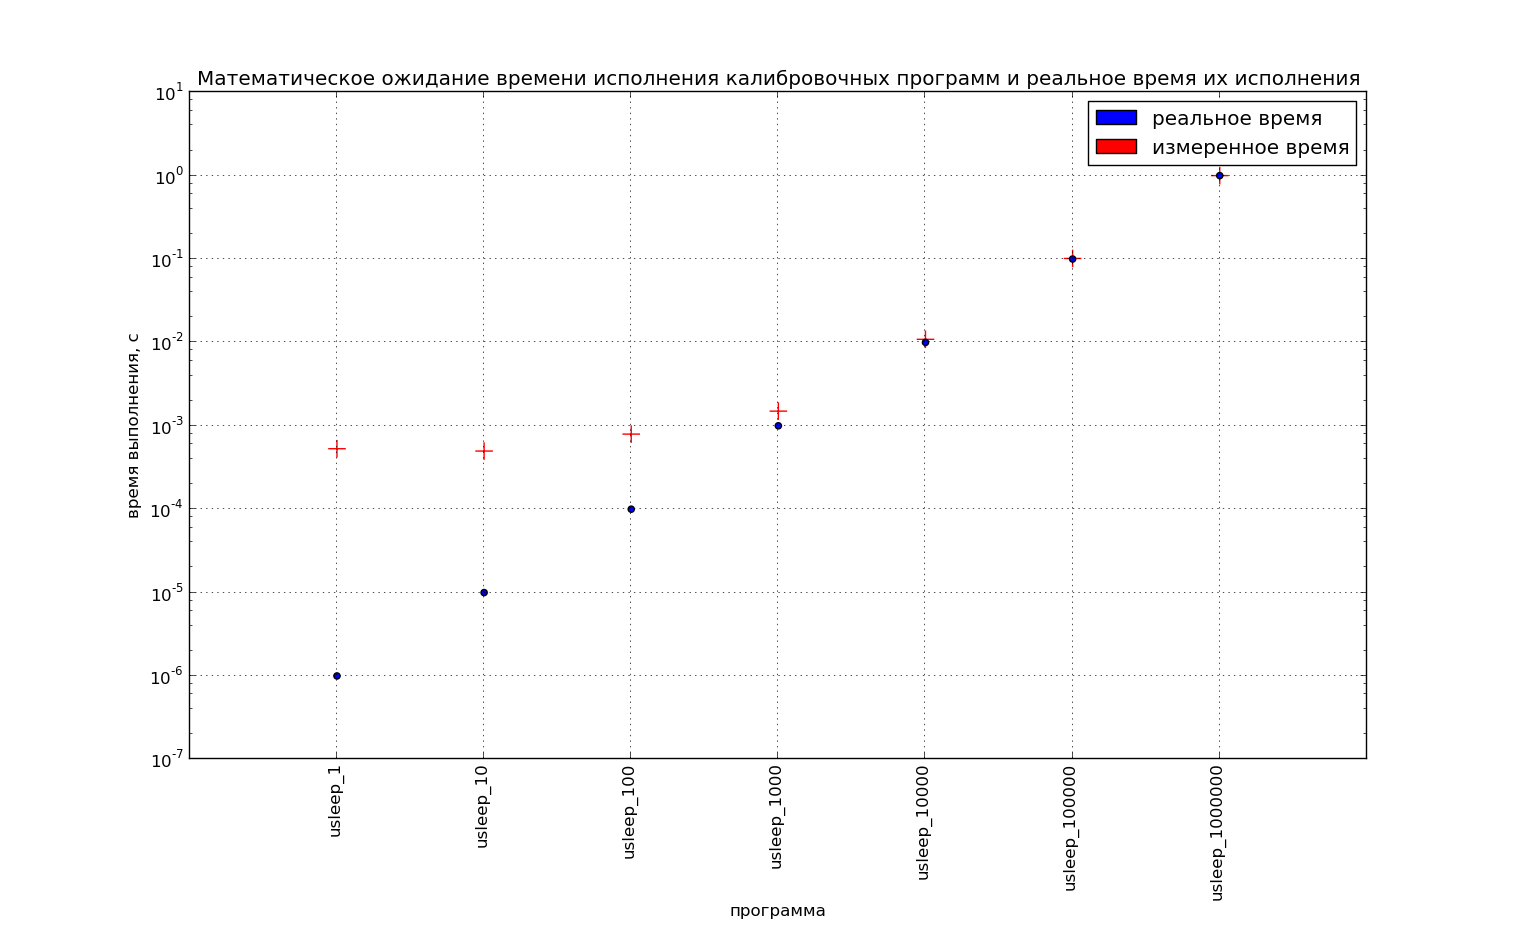
\includegraphics[width=1\linewidth]{calibration-offset}}
    \caption{График измеренного и реального времени исполнения семейства калибровочных программ с учётом накладных расходов}
    \label{img:calibration-offset}
\end{figure}

Далее на рис. \ref{img:default_calibration} приведён текстовый вывод из инструментария результата описанного эксперимента с учётом накладных расходов.

\begin{figure}[H]
    \fontsize{10}{12}
    \begin{verbatim}
        Experiment performed:
            Real time: 0.000001
            Measured time: 0.000531
            Relative error: 530.11
        
        Experiment performed:
            Real time: 0.000010
            Measured time: 0.000498
            Relative error: 48.79
        
        Experiment performed:
            Real time: 0.000100
            Measured time: 0.000795
            Relative error: 6.95
        
        Experiment performed:
            Real time: 0.001000
            Measured time: 0.001499
            Relative error: 0.50
        
        Experiment performed:
            Real time: 0.010000
            Measured time: 0.010893
            Relative error: 0.09
        
        Experiment performed:
            Real time: 0.100000
            Measured time: 0.101603
            Relative error: 0.02
        
        Experiment performed:
            Real time: 1.000000
            Measured time: 1.001015
            Relative error: 0.00
    \end{verbatim}
    \caption{Результат работы программы для описанного выше эксперимента.}
    \label{img:default_calibration}
\end{figure}

Таким образом, инструментарий позволяет производить достаточно точное измерение времени (ошибка в пределах 10\%) для программ, исполняющихся 10 мс и более.


\subsection{Серия экспериментов по сравнению компиляторов GCC и LLVM на тестовом наборе Polybench}
\label{series-llvm-vs-gcc}
На рисунке~\ref{img:gcc-vs-clang} сравнивается время исполнения программ, собранных компиляторами \textit{GCC} и \textit{LLVM} соответственно на уровне оптимизации \texttt{-O2}. Компилятор на этом уровне оптимизации в подавляющем большинстве случаев генерирует наиболее быстрый код (относительно уровней \texttt{-O0} и \texttt{-O1}).

\begin{figure}[!bH]
    \center{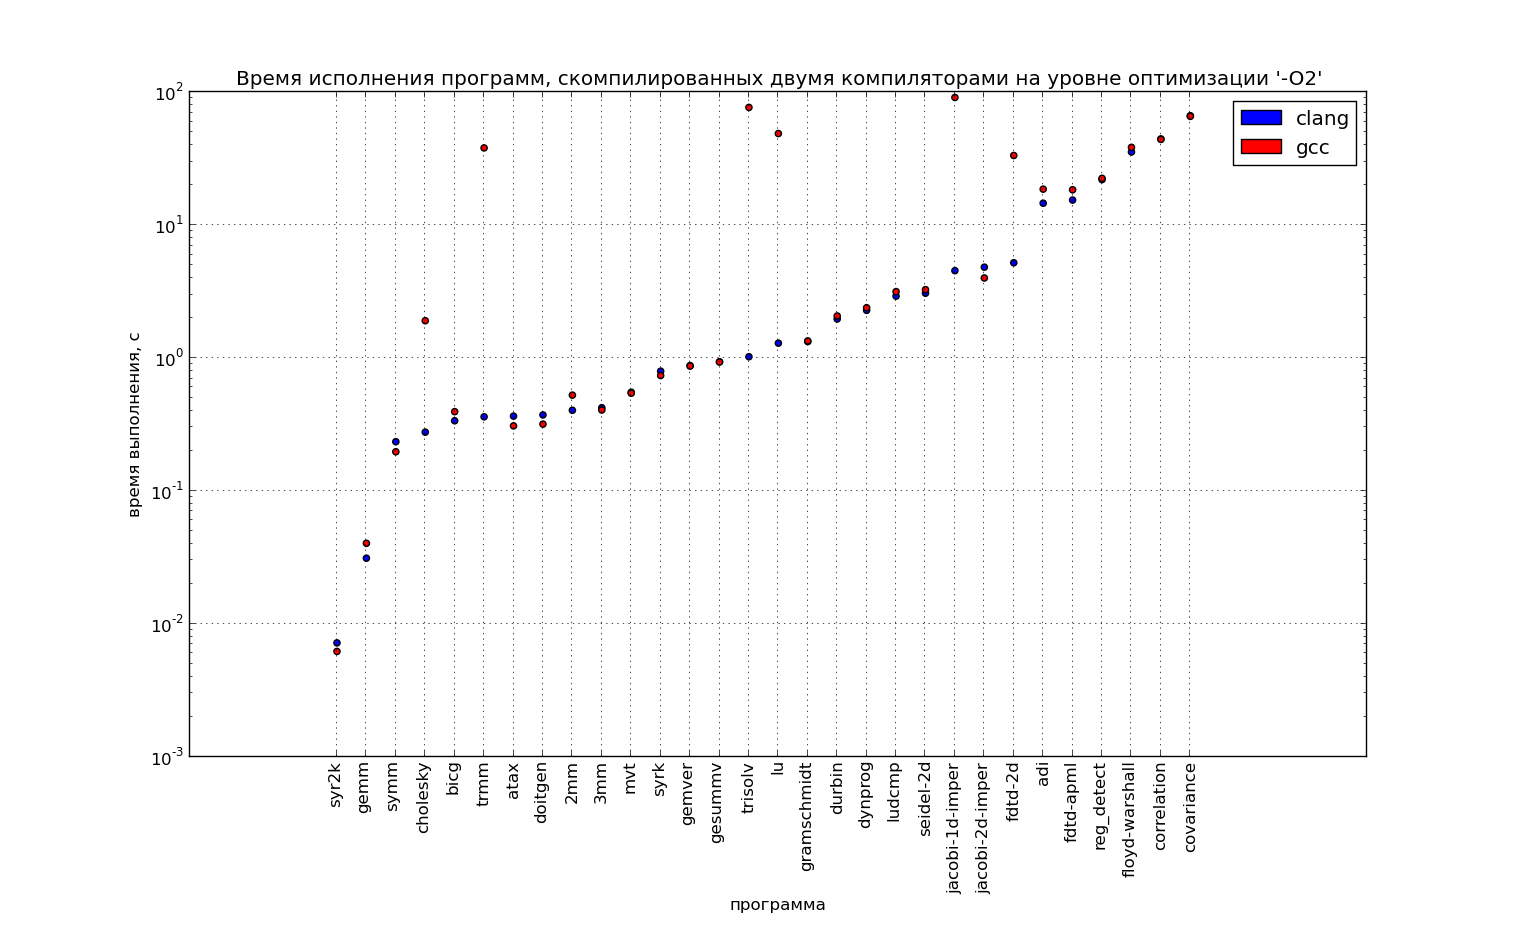
\includegraphics[width=1\linewidth]{gcc-vs-clang}}
    \caption{График времени исполнения программ из набора \textit{Polybench} для двух компиляторов.}
    \label{img:gcc-vs-clang}
\end{figure}

Как мы видим из графика, на большинстве программ оба компилятора показывают примерно одинаковую производительность. Однако на шести программах компилятор \textit{LLVM} серьёзно превосходит \textit{GCC} -- это программы \textit{cholesky, trmm, trisolv, lu, jacobi-1d-imper, fdtd-2d}. Вероятно, \textit{LLVM} использует лучший векторизатор кода, что оказывает большое влияние в этих специфических случаях. В целом, указанные программы относятся к различным классам "--- это программы решения СЛАУ и СДУ. Выяснение конкретных причин этого превосходства выходит за рамки данной работы.

\subsection{Группа серий экспериментов по моделированию и предсказанию производительности программы из набора Polybench на различном аппаратном обеспечении}

Одной из возможностей, предоставляемых инструментарием, является статистический анализ данных серии экспериментов с целью предсказания производительности программ на различном аппаратном обеспечении при различном размере и форме входных данных.

Для этого выберем программу из набора \textit{Polybench}, которую будем анализировать. Критериями выбора являются факторы, приведённые ниже.
\begin{itemize}
    \item Время исполнения программы при различных размерах и формах входных данных должно быть не слишком велико. Поскольку в рамках серии экспериментов программа должна быть исполнена статистически значимое число раз (по крайней мере 100), мы должны выбрать программу с учётом доступных ресурсов машинного времени и общих ресурсов времени, которое можно потратить на исследование.
    \item Время исполнения программы при различных размерах и формах входных данных должно быть не слишком мало. При уменьшении времени однократного исполнения программы погрешность измерения реального времени исполнения возрастает -- до~50\% при времени однократного исполнения 0,001~с (см. раздел~\ref{ssec:series-accuracy}). Поэтому мы должны выбрать программу, которая исполняется секунду или более, для достижения оптимальных результатов. При указанном времени исполнения точность измерения времени достигает как минимум~99\% (раздел \ref{ssec:series-accuracy}).
\end{itemize}

На основании указанных критериев и данных, полученных в рамках серии экспериментов, описанной в разделе \ref{series-llvm-vs-gcc}, выбираем программу \texttt{symm} в качестве анализируемой.

Мы осуществим три серии экспериментов по моделированию и предсказанию производительности программы \texttt{symm} из набора \textit{Polybench}. Они перечислены ниже.
\begin{enumerate}
    \item Первая серия экспериментов характеризуется размерами входных данных $M$ (число столбцов обрабатываемой матрицы) и $N$ (число строк обрабатываемой матрицы), задаваемыми по степенному закону $M = N = 2^x, x = [1;12]$. Таким образом, $M = N \in [2;4096]$.
    \item Вторая серия экспериментов характеризуется размерами входных данных $M$ и $N$, задаваемыми случайно из диапазона [2;2048]: $M = N = rand([2;2048])$, где $rand$ -- функция случайного выбора целого числа из указанного диапазона по равномерному закону распределения. Таким образом, $M = N \in [2;2048]$.
    \item Третья серия экспериментов характеризуется размерами входных данных $M$ и $N$, задаваемыми случайно и независимо из диапазона [2;2048]: $M = rand_1([2;2048]), N = rand_2([2;2048])$, где $rand_i, i \in [1;2]$ -- выборки случайного выбора целого числа из указанного диапазона по равномерному закону распределения (в данном случае выбираются два случайных числа). Таким образом, $M, N \in [2;2048]$.
\end{enumerate}

В каждой серии экспериментов производится обучение трёх предсказателей -- \textit{Earth, Random Forest и k-Nearest Neigbour} -- и последующее предсказание производительности программы \texttt{symm} на различных аппаратных платформах и при различных размерах входных данных. Обучение производится на двух различных моделях -- простейшей (включающей всего один признак из набора экспериментальных данных), и более сложной (включающей в себя до пяти признаков из набора экспериментальных данных). Обучение и предсказание на основе экспериментальных данных производится в системе статистической обработки данных с открытым исходным кодом \textit{Orange}~\cite{orange}.

Хронологически, первой была выполнена серия экспериментов №3 как наиболее сложная, на которой предстояло выбрать надёжный алгоритм выбора признаков, который был бы способен работать и в более простых случаях (в сериях №1 и №2).

Система моделирования и предсказания организована в форме конвейера с ветвлениями, как описано в разделе~\ref{orange-pipeline}.

Рассмотрим результаты выполнения серий экспериментов и моделирования производительности программы \texttt{symm} в каждом случае.


\subsubsection{Серия экспериментов №1}

Результаты сравнения предсказателей показаны на рисунках~\ref{img:series30-Test-Learners-1}~и~\ref{img:series30-Test-Learners-2}.

\begin{figure}[H]
    \begin{center}
            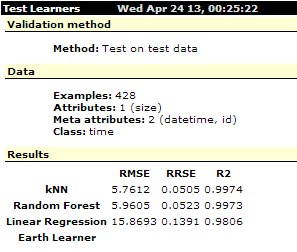
\includegraphics[scale=0.75]{series30-Test-Learners-1}
            \caption{Сравнение предсказателей для модели с одним признаком. Серия~№1.} %% подпись к рисунку
            \label{img:series30-Test-Learners-1} %% метка рисунка для ссылки на него
    \end{center}
\end{figure}

\begin{figure}[H]
    \begin{center}
            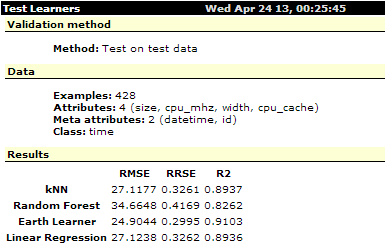
\includegraphics[scale=0.75]{series30-Test-Learners-2}
            \caption{Сравнение предсказателей для модели с четырьмя признаками. Серия~№1.}
            \label{img:series30-Test-Learners-2}
    \end{center}
\end{figure}

Как можно видеть на рисунках, в этой серии экспериментов, при использовании модели с одним признаком, все предсказатели показывают примерно одинаково высокие значения метрики $R2 \approx 0,99$, однако \textit{kNN} и \textit{RF} показывают значительно меньшие значения метрики RRSE, что означает более точное предсказание. Это отличный результат.

Из-за внутренней ошибки системы \textit{Orange} проверить предсказатель \textit{Earth} на модели с одним признаком не удалось.

\begin{figure}[H]
    \begin{center}
        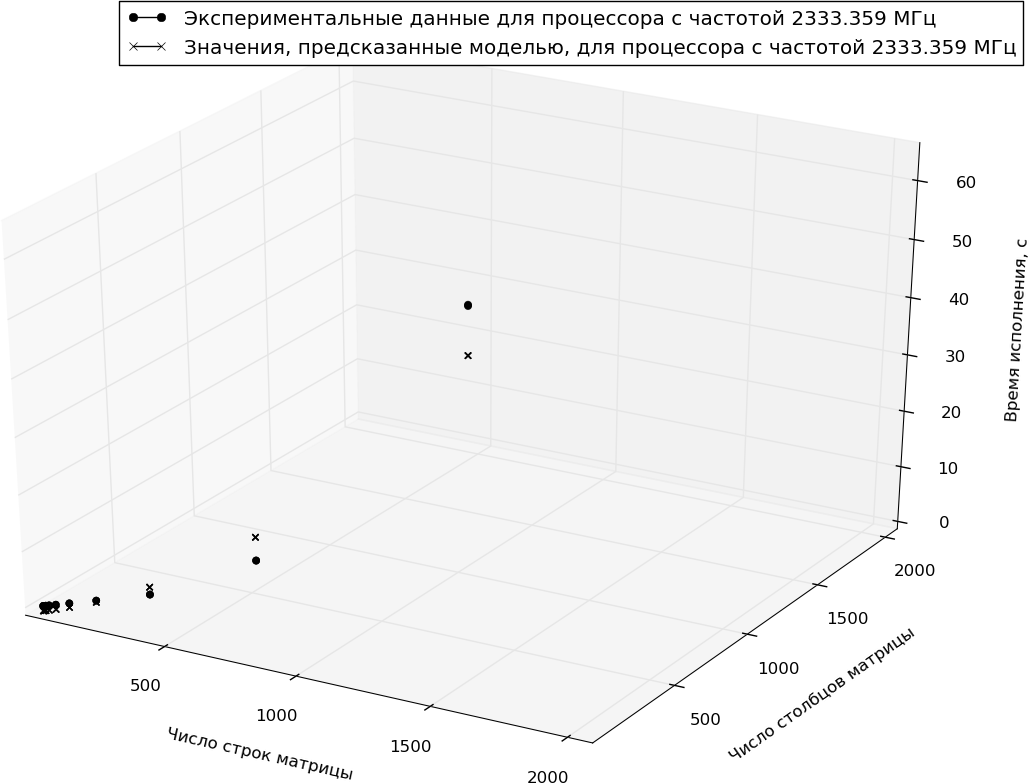
\includegraphics[scale=0.5]{powers-predictions-5f-earth-2333-0}
        \caption{Экспериментальные и предсказанные данные для процессора с частотой 2333~МГц. Серия~№1. Предсказатель \textit{Earth}.}
        \label{img:powers-predictions-5f-earth-2333-0}
    \end{center}
\end{figure}

При использовании модели с четырьмя признаками предсказатель \textit{Earth} превосходит все остальные по значениям метрик $RRSE$ и $R2$, и показывает $R2 \approx 0,91$, что следует признать хорошим результатом.

\begin{figure}[H]
    \begin{center}
        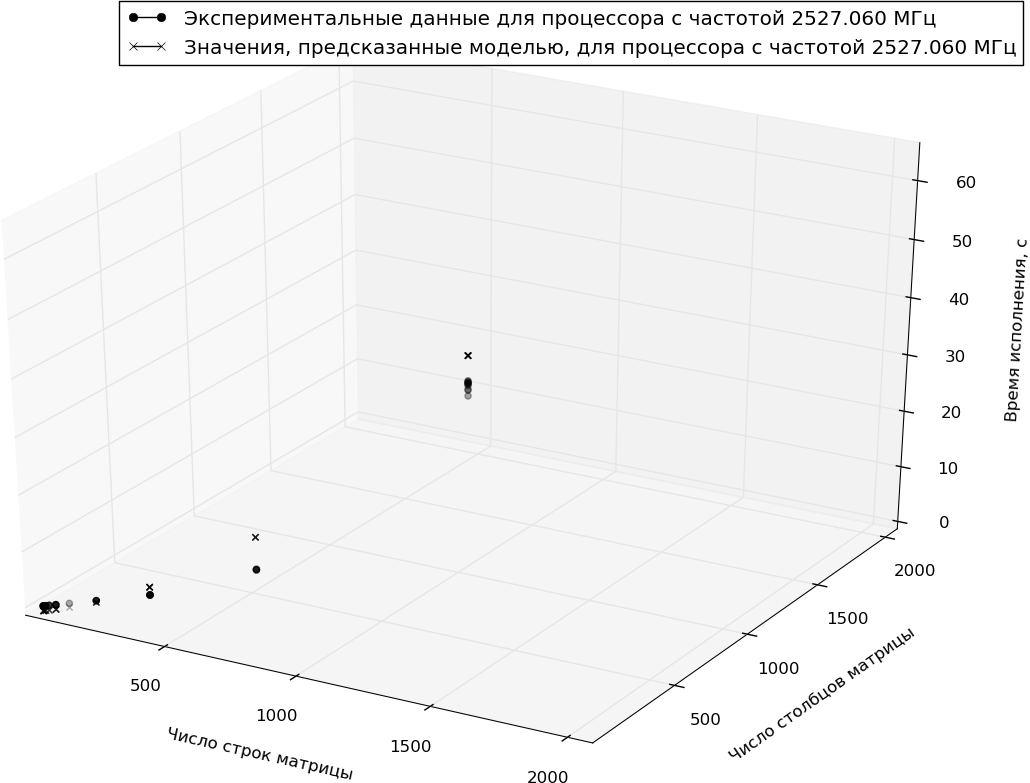
\includegraphics[scale=0.5]{powers-predictions-5f-earth-2527-0}
        \caption{Экспериментальные и предсказанные данные для процессора с частотой 2527~МГц. Серия~№1. Предсказатель \textit{Earth}.}
        \label{img:powers-predictions-5f-earth-2527-0}
    \end{center}
\end{figure}

На рисунках~\ref{img:powers-predictions-5f-earth-2333-0},\,\ref{img:powers-predictions-5f-earth-2527-0},\,\ref{img:powers-predictions-5f-earth-2666-0} приведены графики лучшего предсказателя для модели с четырьмя признаками "--- \textit{Earth Learner} "--- по данным для каждого из трёх процессоров.

\begin{figure}[H]
    \begin{center}
        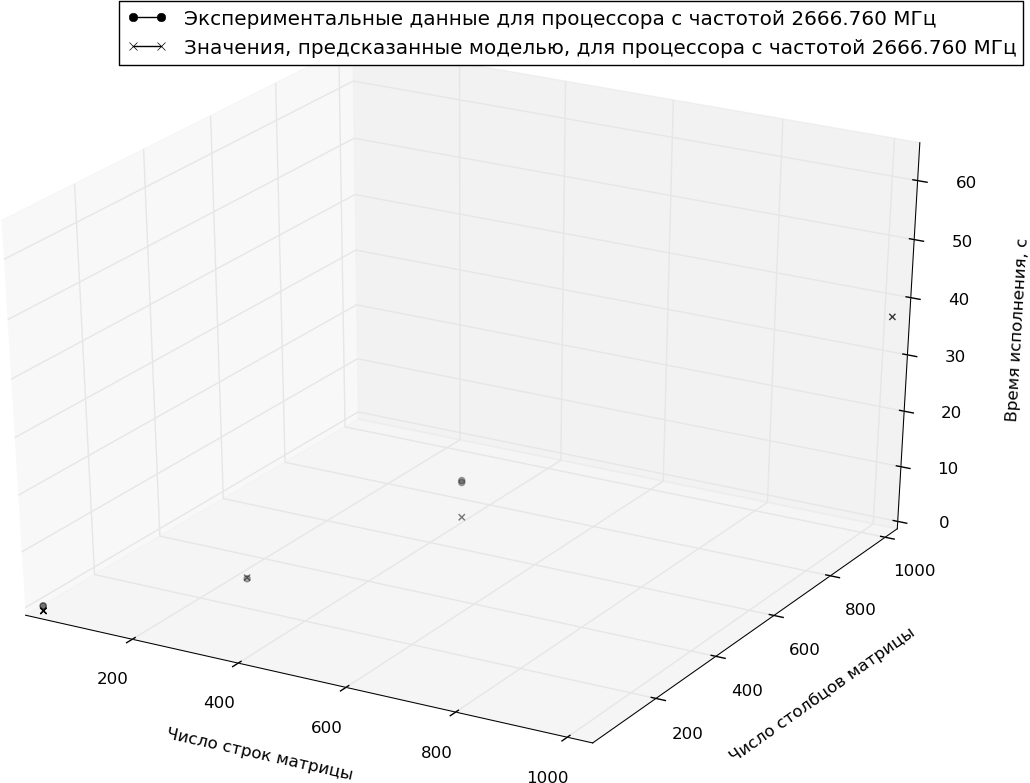
\includegraphics[scale=0.5]{powers-predictions-5f-earth-2666-0}
        \caption{Экспериментальные и предсказанные данные для процессора с частотой 2667~МГц. Серия~№1. Предсказатель \textit{Earth}.}
        \label{img:powers-predictions-5f-earth-2666-0}
    \end{center}
\end{figure}

Как мы видим на графиках, для всех трёх процессоров предсказания находятся достаточно близко к реально полученным данным. Это говорит о хорошей способности модели обобщать, то есть выводить наиболее простой закон получения неизвестного значения времени исполнения по известным значениям всех остальных свойств эксперимента. При этом не наблюдается явления переобучения, которое состоит в том, что модель показывает отличные результаты на учебной выборке и низкие результаты на проверочной.


\subsubsection{Серия экспериментов №2}

Результаты сравнения предсказателей показаны на рисунках~\ref{img:series20-Test-Learners-1}~и~\ref{img:series20-Test-Learners-2}.

\begin{figure}[H]
    \begin{center}
            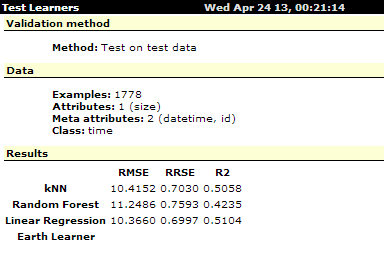
\includegraphics[scale=0.75]{series20-Test-Learners-1}
            \caption{Сравнение предсказателей для модели с одним признаком. Серия~№2.} %% подпись к рисунку
            \label{img:series20-Test-Learners-1} %% метка рисунка для ссылки на него
    \end{center}
\end{figure}

\begin{figure}[H]
    \begin{center}
            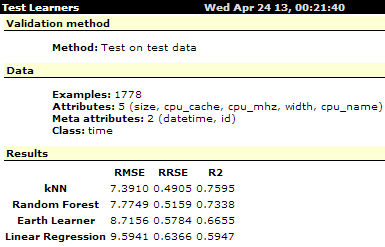
\includegraphics[scale=0.75]{series20-Test-Learners-2}
            \caption{Сравнение предсказателей для модели с четырьмя признаками. Серия~№2.}
            \label{img:series20-Test-Learners-2}
    \end{center}
\end{figure}

В этой серии экспериментов результаты предсказания ожидаемо хуже. Значения метрики $R2$ достигают только $\approx 0,51$ для модели с одним признаком и $\approx 0,76$ для модели с пятью признаками.

Следует отметить, что в случае модели с одним признаком ни один из предсказателей не показал результатов лучше, чем образцовый предсказатель "--- линейная регрессия. Это говорит о неспособности модели предоставить данные для адекватной работы предсказателей, более сложных, чем линейный. Эта модель не может качественно представлять данные серии экспериментов~№2.

\begin{figure}[H]
    \begin{center}
        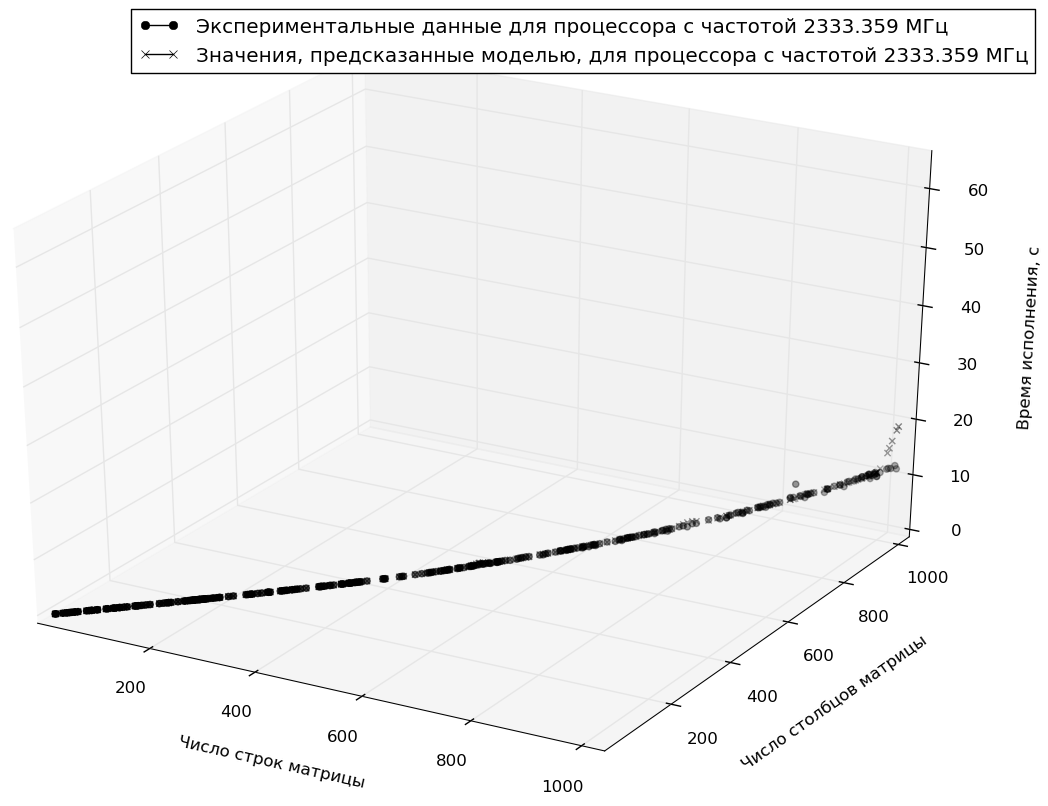
\includegraphics[scale=0.5]{uniform-predictions-5f-knn-2333-0}
        \caption{Экспериментальные и предсказанные данные для процессора с частотой 2333~МГц. Серия~№2. Предсказатель \textit{kNN}.}
        \label{img:uniform-predictions-5f-knn-2333-0}
    \end{center}
\end{figure}

При использовании модели с пятью признаками наилучший результат показал предсказатель \textit{kNN}: $RRSE = 0,4905; R2 = 0,7595$. Однако, этот результат значительно ниже, чем полученный в серии~№1. Давайте посмотрим на графики предсказаний (рисунки~\ref{img:uniform-predictions-5f-knn-2333-0},~\ref{img:uniform-predictions-5f-knn-2527-0},~\ref{img:uniform-predictions-5f-knn-2666-0}) для определения источника проблем.

\begin{figure}[H]
    \begin{center}
        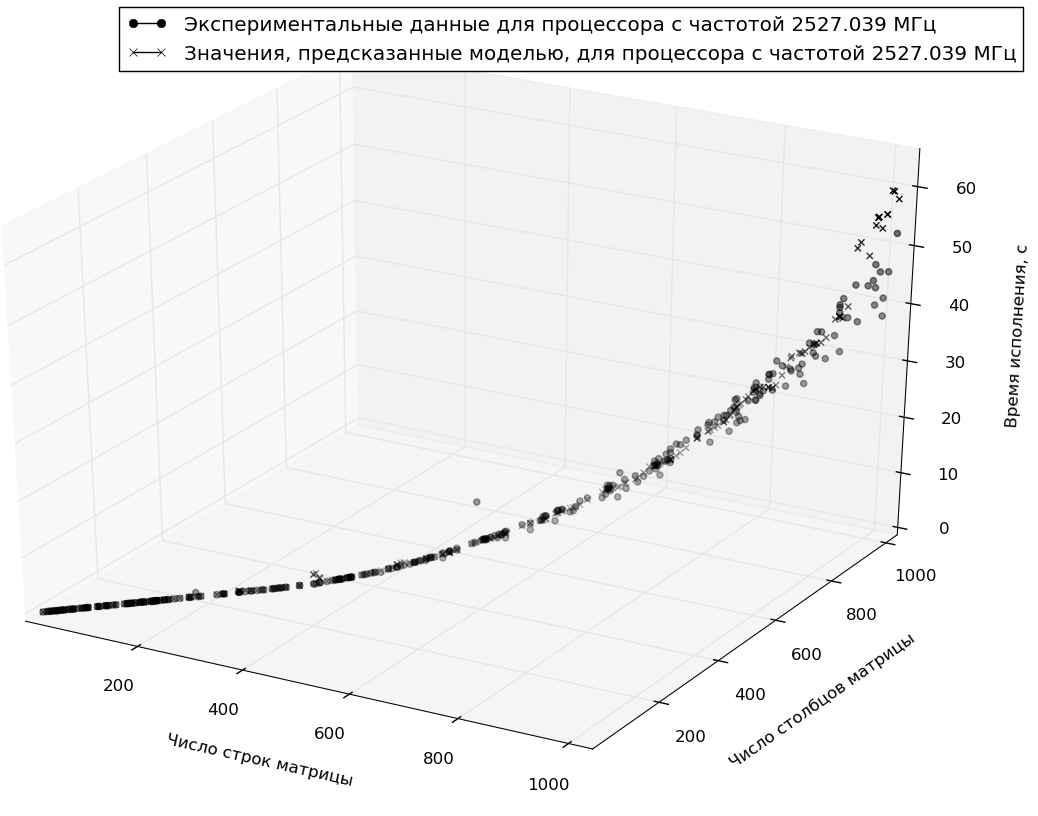
\includegraphics[scale=0.5]{uniform-predictions-5f-knn-2527-0}
        \caption{Экспериментальные и предсказанные данные для процессора с частотой 2527~МГц. Серия~№2. Предсказатель \textit{kNN}.}
        \label{img:uniform-predictions-5f-knn-2527-0}
    \end{center}
\end{figure}

Первые два графика показывают довольно адекватные в целом предсказания: только на правом крае графика, при больших значениях размера матрицы, наблюдается небольшое расхождение. Однако для последнего процессора, Intel Xeon 2,66~ГГц, модель начинает предсказывать неадекватные значения времени исполнения уже начиная с размера матрицы $400 \times 400$. Можно заметить, что часть экспериментальных данных для матриц больших размеров располагается на показательной кривой, а часть "--- на практически линейном участке, причём линейная часть находится в диапазоне очень маленьких времён исполнения. Это является артефактом проведения эксперимента на виртуальном сервере, который может не иметь эксклюзивного доступа к аппаратному обеспечению физического сервера, на котором он запущен. Судя по разбросу данных, периодически происходило переключение сервера в режим высокой производительности, при котором он получал полный доступ к аппаратным ресурсам, в результате чего исследуемая программа исполнялась за значительно меньшее время. Б\'{о}льшую же часть времени сервер мог использовать только часть ресурсов, поэтому время исполнения в основном находится на верхней, показательной, кривой.

\begin{figure}[H]
    \begin{center}
        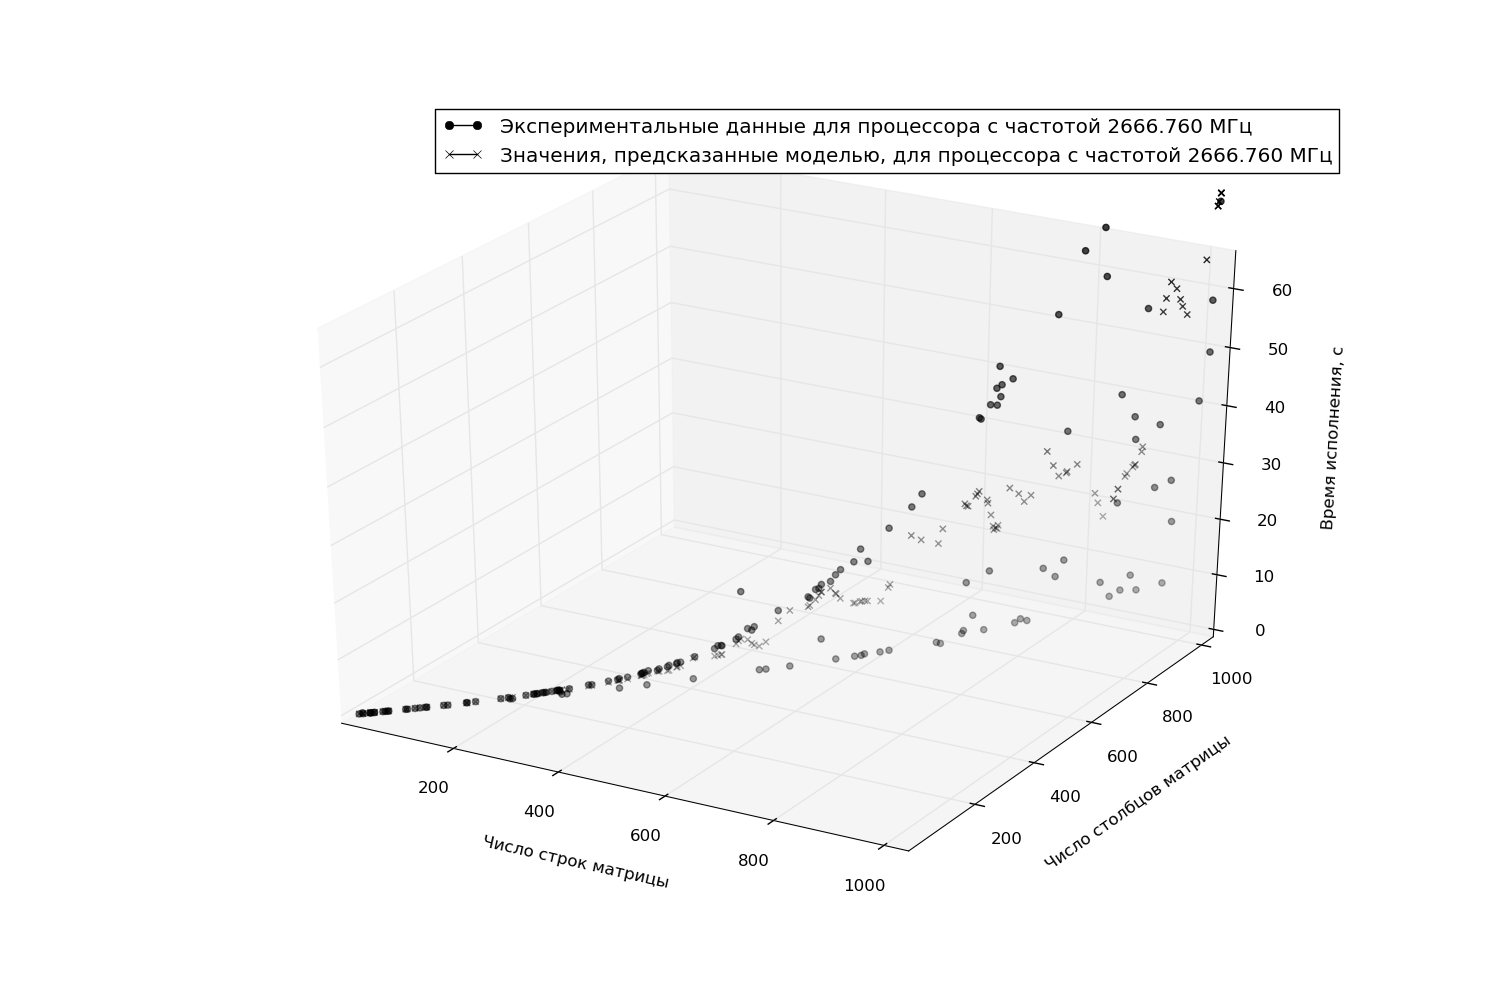
\includegraphics[scale=0.5]{uniform-predictions-5f-knn-2666-0}
        \caption{Экспериментальные и предсказанные данные для процессора с частотой 2667~МГц. Серия~№2. Предсказатель \textit{kNN}.}
        \label{img:uniform-predictions-5f-knn-2666-0}
    \end{center}
\end{figure}

Этим объясняется и неадекватность предсказаний для последнего процессора "--- взглянув на графики, можно увидеть, что предсказатель попытался объяснить и наличие точек на показательной кривой, и на более низком линейном участке, в результате чего кривая предсказаний оказалась посередине и представляет собой сильно зашумленную, неадекватную кривую, состоящую из нескольких линейных участков.

Причиной неадекватности модели в данном случае стало отсутствие в наборе данных каких-то свойств, указывающих на то, что машина является виртуальным сервером и ей могут быть не доступны все ресурсы реального сервера. Проблемой здесь оказалось то, что модулю опроса аппаратного обеспечения сообщаются именно данные о реальном сервере, а не о текущих доступных ресурсах, и нет простого способа распознать использование виртуализации.


\subsubsection{Серия экспериментов №3}

Результаты сравнения предсказателей показаны на рисунках~\ref{img:series10-Test-Learners-1}~и~\ref{img:series10-Test-Learners-2}.

\begin{figure}[H]
    \begin{center}
        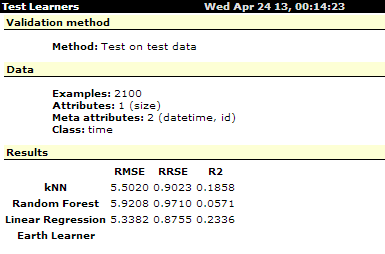
\includegraphics[scale=0.75]{series10-Test-Learners-1}
        \caption{Сравнение предсказателей для модели с одним признаком. Серия~№3.} %% подпись к рисунку
        \label{img:series10-Test-Learners-1} %% метка рисунка для ссылки на него
    \end{center}
\end{figure}

\begin{figure}[H]
    \begin{center}
        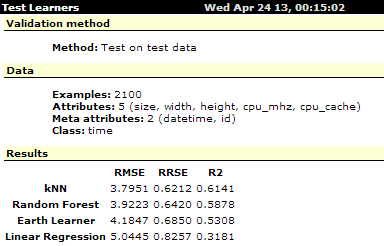
\includegraphics[scale=0.75]{series10-Test-Learners-2}
        \caption{Сравнение предсказателей для модели с четырьмя признаками. Серия~№3.}
        \label{img:series10-Test-Learners-2}
    \end{center}
\end{figure}

В этой серии экспериментов предсказания оказались наименее точными.

Модель с одним признаком оказалась неспособной давать адекватные предсказания, поскольку все предсказатели показали результаты хуже образцового. Линейная регрессия же показала результат с значением метрики $R2 = 0,2336$, что является неудовлетворительным результатом. В реальных условиях модель с одним признаком оказалась непригодной для использования.

Для модели с пятью признаками наилучшие результаты снова показал предсказатель \textit{kNN}, таким образом показав своё превосходство в случаях, когда эксперименты проводятся в более непредсказуемых условиях. Его значения метрик $RRSE = 0,6212; R2 = 0,6141$. Это удовлетворительный результат, учитывая, что фильтрация данных с целью удаления шума не производилась.

\begin{figure}[H]
    \begin{center}
        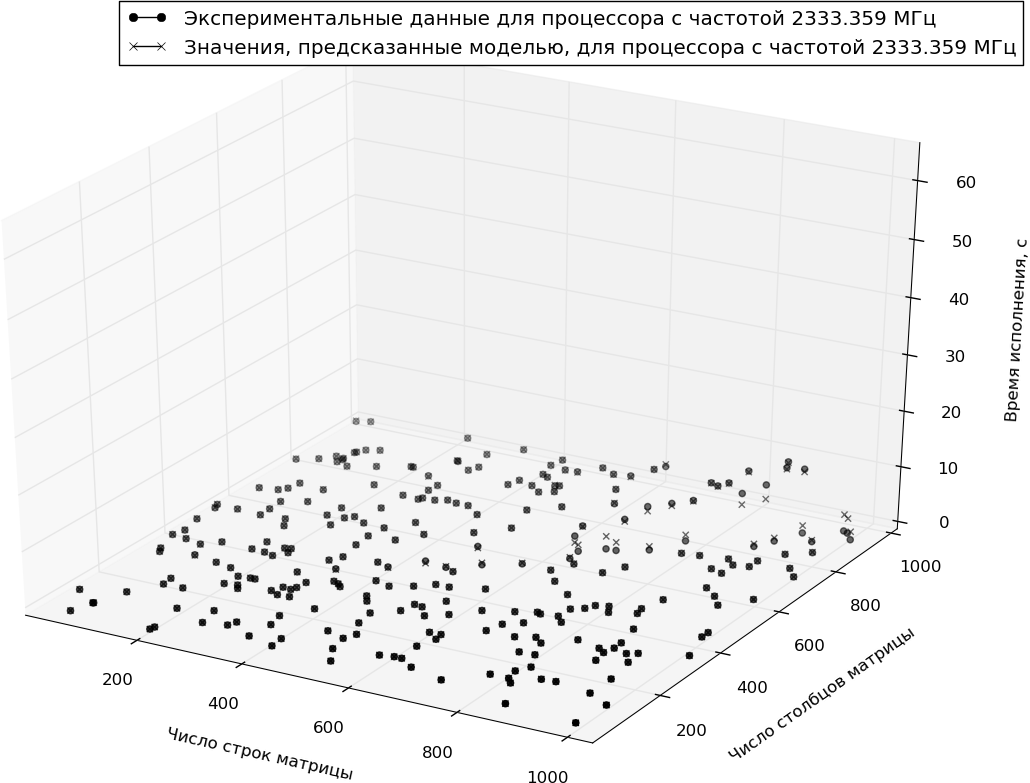
\includegraphics[scale=0.5]{predictions-5f-knn-2333-0}
        \caption{Экспериментальные и предсказанные данные для процессора с частотой 2333~МГц. Серия~№3. Предсказатель \textit{kNN}.}
        \label{img:predictions-5f-knn-2333-0}
    \end{center}
\end{figure}

Давайте посмотрим на графики предсказаний (рисунки~\ref{img:predictions-5f-knn-2333-0},~\ref{img:predictions-5f-knn-2527-0},~\ref{img:predictions-5f-knn-2666-0}) для определения сложностей, с которыми столкнулся предсказатель.

\begin{figure}[H]
    \begin{center}
        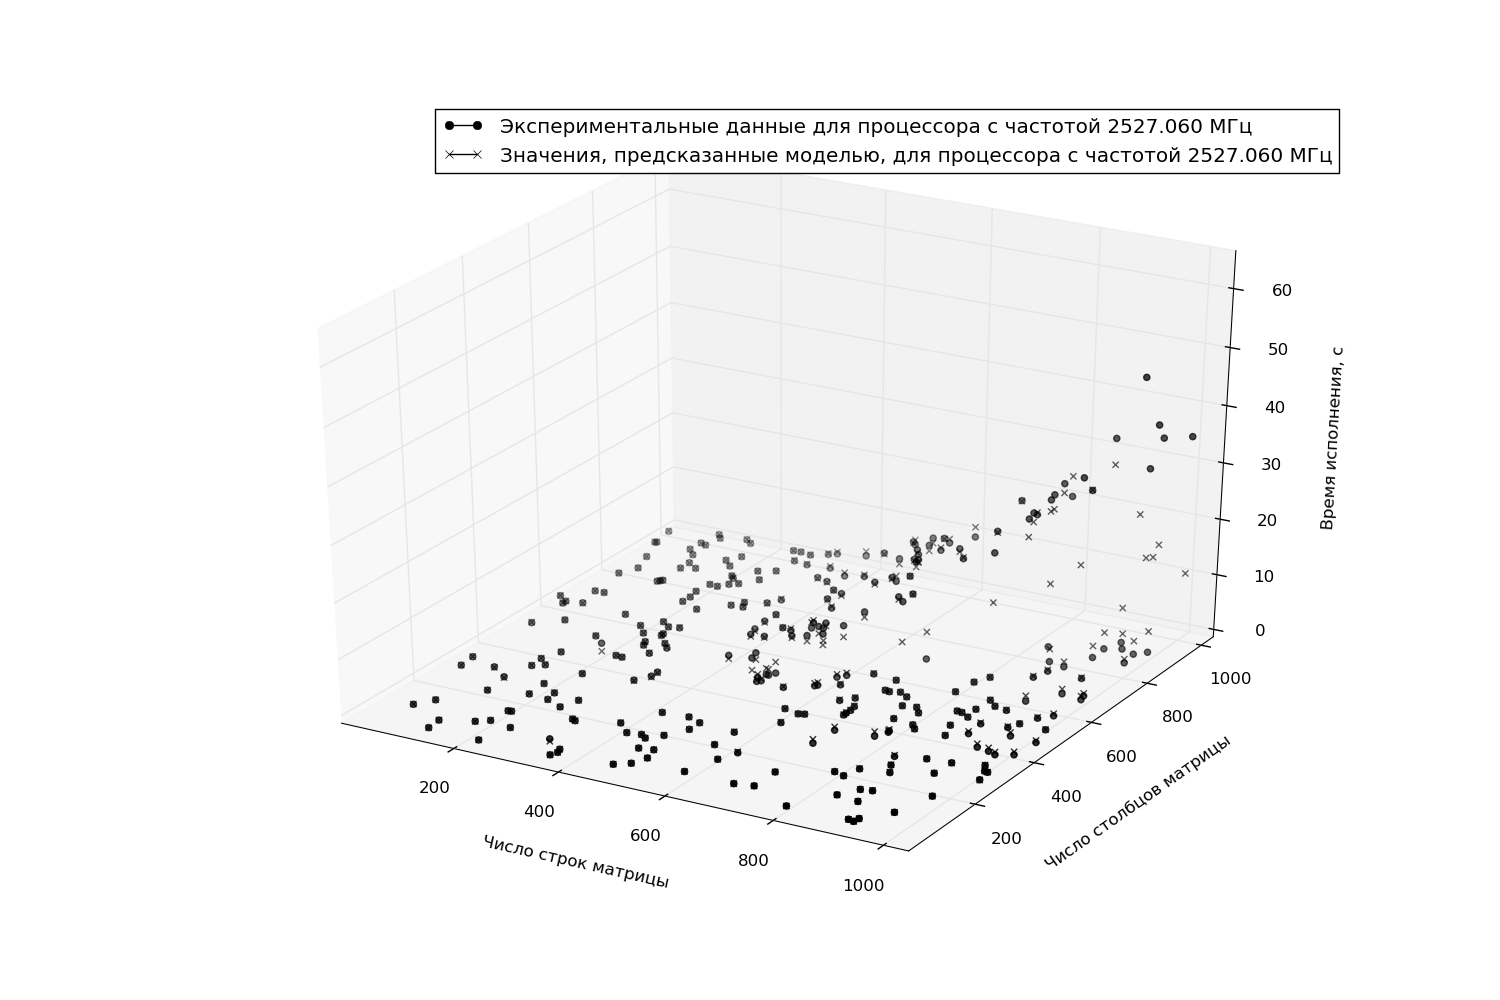
\includegraphics[scale=0.5]{predictions-5f-knn-2527-0}
        \caption{Экспериментальные и предсказанные данные для процессора с частотой 2527~МГц. Серия~№3. Предсказатель \textit{kNN}.}
        \label{img:predictions-5f-knn-2527-0}
    \end{center}
\end{figure}

Поскольку графики являются трёхмерными, выявить вид предсказывающей кривой гораздо сложнее. Можно сказать, что предсказатель страдает от переобучения, поскольку большая часть значений времени оказалась сильно зашумлёнными, минимально возможными к измерению значениями. Из-за этого их колебания очень велики и в ряде случаев из-за артефактов измерения значения времени аномально близки к нулю или даже отрицательны. Это очевидно снижает предсказывающие способности модели, поскольку она производит попытки объяснить наличие зашумленных данных.

\begin{figure}[H]
    \begin{center}
        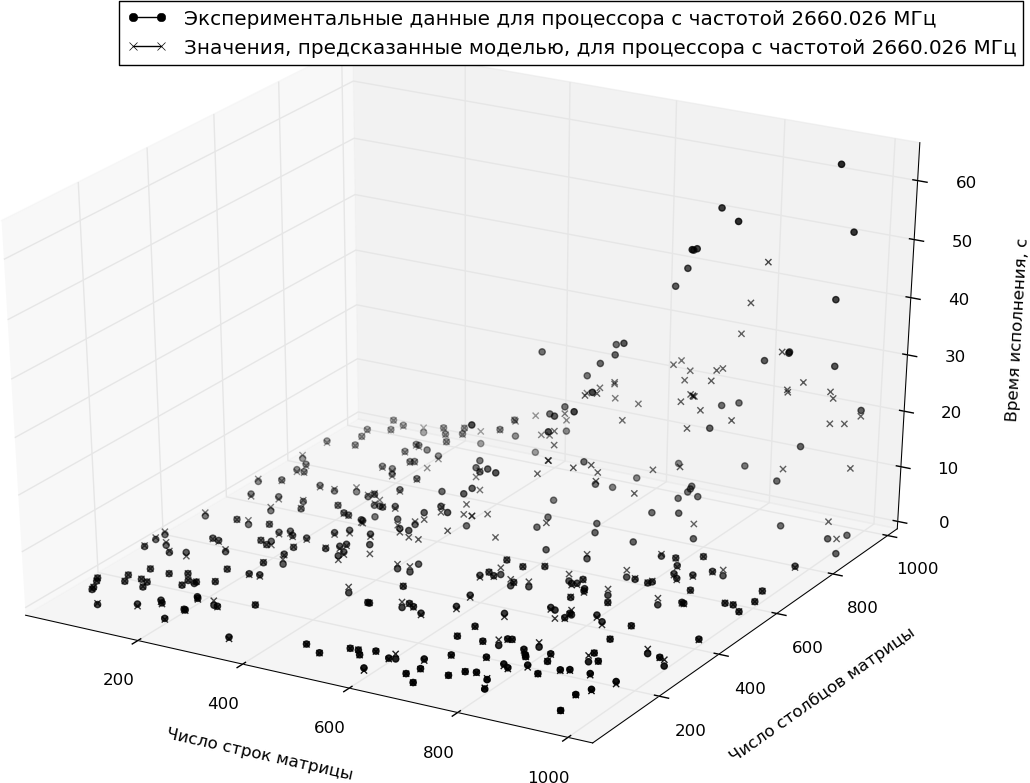
\includegraphics[scale=0.5]{predictions-5f-knn-2666-0}
        \caption{Экспериментальные и предсказанные данные для процессора с частотой 2667~МГц. Серия~№3. Предсказатель \textit{kNN}.}
        \label{img:predictions-5f-knn-2666-0}
    \end{center}
\end{figure}

Вторым фактором является само по себе преобладание предельно коротких запусков программы. Это ведёт к тому, что вероятность возникновения маленьких времён исполнения в результате предсказания возрастает, поскольку в учебном наборе преобладают короткие запуски.

Обе эти проблемы частично решаются фильтрацией шумных результатов, однако определение критериев, по которым измеренное значение можно считать шумом, является не тривиальной задачей и выходит за рамки этой работы.


\subsection{Выводы}
В рамках оценки эффективности разработанного программного продукта было произведено несколько серий экспериментов, в ходе которых была доказана возможность решать задачу статистического анализа производительности программ на различном аппаратном обеспечении с помощью инструментария.